%%%%%%%%%%%%%%%%%%%%%%%%%%%%%%%%%%%%%%
% One Column
%%%%%%%%%%%%%%%%%%%%%%%%%%%%%%%%%%%%%%
\documentclass[smallabstract,smallcaptions]{dccpaper}

\usepackage{epsfig}
\usepackage{epstopdf}
\usepackage{citesort}
\usepackage{amsmath}
\usepackage{amssymb}
\usepackage{color}
\usepackage{url}

\newlength{\figurewidth}
\newlength{\smallfigurewidth}


%%%%%%%%%%%%%%%%%%%%%%%%%%%%%%%%%%%%%%
% One Column
%%%%%%%%%%%%%%%%%%%%%%%%%%%%%%%%%%%%%%
\setlength{\smallfigurewidth}{2.75in}
\setlength{\figurewidth}{6in}

\begin{document}

\title
{\large
\textbf{Universal Rate-Distortion Analysis for Various Source Distributions}
}

\author{%
Shengbin Meng, Jun Sun$^{\ast}$, Yizhou Duan, and Zongming Guo\\[0.5em]
{\small\begin{minipage}{\linewidth}\begin{center}
\begin{tabular}{ccc}
Institution of Computer Science and Technology, \\
Peking University, Beijing, 100086, China\\
\url{{mengshengbin, sunjun, duanyizhou, guozongming}@pku.edu.cn}
\end{tabular}
\end{center}\end{minipage}}
}

\maketitle
\thispagestyle{empty}

\begin{abstract}
This paper studies the complex Rate-Distortion (R-D) analysis problem from a universal perspective. For various probability distributions that have been used to describe real source signals, common properties and principles are revealed and validated based on the dead-zone plus uniform threshold scalar quantization with nearly-uniform reconstruction quantizer (DZ+UTSQ/NURQ) scheme that is adopted by latest image/video coding standards. First, it is observed and mathematically proved that, for any source distribution that can be expressed as the product of a Scaling Factor (SF) and its remaining part, SF does not affect the derivative of its R-D function. This universal property brings new insight and inspiration to R-D modeling, and can assist in important applications such as rate control, fast R-D optimization, etc. Second, finer and efficient DZ+UTSQ/NURQ design principles are deduced for various sources, which can be used to conveniently guile the parameter selection of practical quantizers and evaluate the R-D performance of them. Simulation experiments for Cauchy distribution, which still lacks thorough analysis in the literature, are present to conform the general findings, which are increasingly valuable as more sophisticated source is produced in practice and a specific distribution becomes more limited in use.
\end{abstract}

\section{Introduction}

\let\thefootnote\relax\footnotetext{* is the corresponding author.}

The lossy compression of digital video/image data finally leads to transform-based coding of residuals obtained from intra or inter-frame prediction \cite{Sullivan_IEEE2005}. The coefficients of the transform, DCT or alike in most cases, are processed through quantization and entropy coding, from which bits are produced and distortion is introduced. The rate of bits coming from the entropy coder and the distortion caused by quantization are two aspects that measure the efficiency of the compression. In this scenario, the transform coefficients are referred to as source signals, and the whole process belongs to the source coding realm.

As one of the fundamental issues of source coding, rate-distortion (R-D) analysis has attracted considerable research attentions. R-D analysis focuses on studying the essential property and relationship between rate and distortion of the source signals under applicable quantization technologies. In practice, the statistical properties of the source signals are typically characterized by source distributions, whereas the transform-based entropy-constrained scalar quantization is the most extensively applied quantization technology in current source coding standards \cite{Hang_TCSVT1997}. Therefore, R-D analysis is generally represented by studying the R-D relationship and R-D performance of applying certain scalar quantizer to a given source distribution.

On one hand, to evaluate the attainable optimum R-D performance, for some given source distributions, different types of scalar quantizers have been analyzed and compared \cite{Sullivan_TIT1996}, among which the dead-zone plus uniform threshold quantizer (DZ+UTSQ) with nearly-uniform reconstruction quantizer (NURQ) is recommended and now applied in all the major international video/image coding standards \cite{Sullivan_VCIP2005}. On the other hand, regards to which distribution is most appropriate to accurately model the real source signals (DCT coefficients) in video/image coding, no consensus is ever reached. Some researchers prefer Gaussian \cite{Pratt_Wiley1978}, Laplacian \cite{Smooth_SPIE1996}, or their parametric family Generalized Gaussian distribution (GGD) \cite{Farvardin_TIT1984} \cite{Sun_TCSVT2009}, while others claim that Cauchy distribution is a better choice \cite{Kamaci_TCSVT2005} \cite{Rodríguez_TCSVT_2010}. Proposals for more sophisticated models such as mixed Gaussian \cite{Eude_ICASSP1994}, Bernoulli GGD \cite{Fraysse_TIT2009}, multiple Laplacian \cite{Lee_TCSVT2014} are also reported. Among these various distributions, R-D analysis for the Gaussian family has been thoroughly conducted \cite{Sun_2013TIP}. For example, performance of the DZ+UTSQ/NURQ quantizer is well investigated for Laplacian and Gaussian by Gary in \cite{Sullivan_VCIP2005}. However, for Cauchy and other more complex distributions, the existing conclusions are still quite limited and are mostly based on empirical approach which may lack accuracy and robustness.

In this paper, instead of focusing on the R-D analysis of specific source distribution, we try to find the common rules existing for various different source distributions. The main contributions of this study is to provide insights and assistance in R-D modeling and quantizer design for real coding applications, regardless of the distribution form of the source. First, the property of general sources under DZ+UTSQ/NURQ is discovered to identify the irrelevance of the so called "scaling factor" to the derivative R-D function, which properly reduces the complexity of the R-D modeling problem. Second, by taking the revealed properties into account, efficient DZ+UTSQ/NURQ design principles are deduced for various sources, which can be used to conveniently guile the parameter selection of practical quantizers and evaluate the R-D performance of them.
The general findings in this paper are validated with the Cauchy distribution, and it is noted that they are also consistent with existing conclusions of other distributions.

The rest of this paper is organized as follows. In Section 2, the background knowledge of R-D analysis problem is briefly introduced. On this basis, Section 3 and Section 4 respectively discusses the general R-D property and quantizer design principle that applies to various source distributions, with both mathematical derivation and simulated validation. Finally, concluding remarks are given in Section 5.

\section{Background Knowledge}

\subsection{Scaling Factor of General Source Distributions}
Let $p(x)$ be the Probabilistic Density Function (PDF) of an arbitrarily given source distribution, and $c>0$ is one of its parameters. If there exists a function $q(x)$ irrelevant to $c$ satisfying:
\begin{equation}
\label{equ:SF}
p(x)=\frac{1}{c} q(\frac{x}{c}),\qquad \forall x \in \mathbf{R},
\end{equation}
the parameter $c$ is defined as a \emph{Scaling Factor} (SF) of $p(x)$, and $q(x)$ is defined as the \emph{Remaining Part} (RP) irrelevant to $c$.

SF only stretches or compresses the PDF along axis without affecting the shape of PDF. According to (\ref{equ:SF}), some typical zero-mean source distributions, e.g. GGD, GCD, and Cauchy distribution are expressed in terms of SF and RP in Table \ref{tab:SF}. %The effect of SF on these source distributions are illustrated in Fig.~\ref{fig_1:GGD_scale}, Fig.~\ref{fig_2:GCD_scale} and Fig.~\ref{fig_3:Cauchy_scale}, respectively.

\begin{table}[htp]
	\begin{center}
	\caption{\label{tab:SF}%
	The SF and RP of Some Typical Zero-Mean Source Distributions}
	\vspace{-5pt}
	{
		\renewcommand{\arraystretch}{1.7}
		\begin{tabular}{cccc}
			Source Distribution & PDF: $p(x)$ & SF: $c$ & RP: $q(x)$ \\
			\hline
			GGD & $\frac{g_1(\alpha)}{\beta}\exp\left(-\left(g_2(\alpha)\frac{|x|}{\beta}\right)^\alpha\right)$ & $\beta$ & $g_1(\alpha)\exp\left(-\left(g_2(\alpha)|x|\right)^\alpha\right)$ \\
			GCD & $\frac{k\Gamma(\frac{2}{k})}{2(\Gamma(\frac{1}{k}))^2} h\left(h^k + |x|^k\right)^{-\frac{2}{k}}$ & $h$ & $\frac{k\Gamma(\frac{2}{k})}{2(\Gamma(\frac{1}{k}))^2} \left(1+|x|^k\right)^{-\frac{2}{k}}$ \\
			Cauchy & $\frac{1}{\pi} \frac{\mu}{\mu^2+x^2}$ &  $\mu$ & $\frac{1}{\pi (1+x^2)}$ \\
			\hline
		\end{tabular}
	}
	\vspace{-5pt}
	\end{center}
\end{table}

% \begin{figure}[t]
% %\setlength{\abovecaptionskip}{0pt}
% %\setlength{\belowcaptionskip}{0pt}
% \centering
% \includegraphics[width = 0.7\linewidth]{gray/basic_GGD_scale}\\
% \caption{\label{fig_1:GGD_scale}%
% The effect of SF on GGD ($\alpha = 1, \beta \in \{0.1, 0.2, 0.5, 1\}$)}
% \includegraphics[width = 0.7\linewidth]{gray/basic_GCD_scale}\\
% \caption{\label{fig_2:GCD_scale}%
% The effect of SF on GGD ($k = 1, h \in \{0.1, 0.2, 0.5, 1\}$)}
% \includegraphics[width = 0.7\linewidth]{gray/basic_Cauchy}\\
% \caption{\label{fig_3:Cauchy_scale}%
% The effect of SF on Cauchy Distribution ($\mu \in \{0.1, 0.2, 0.5, 1\}$)}
% \end{figure}

\subsection{DZ+UTSQ/NURQ Scheme}
DZ+UTSQ/NURQ scheme is illustrated in Fig. \ref{fig:DZ+UTSQ_NURQ}, which consists of DZ+UTSQ classification process and NURQ reconstruction process, both are symmetric about zero. In classification, each input signal is rounded to an integer quantization index according to its \emph{quantization interval} $I$, which is determined by the \emph{quantization threshold} $T$. Then in reconstruction, each quantization index is mapped to a real-valued \emph{reconstruction level} $R$ as the output. For the quantization index $k$, the corresponding $kth$ quantization interval $I_{k}$ of general DZ+UTSQ/NURQ is denoted by:
\begin{equation}
\label{equ:interval}
I_{k}=\left\{ \begin{array}{ll}
(T_{-1}, T_{1}),         & k = 0 \\
{[T_{k}, T_{k+1})},        & k \ge 1 \\
(T_{-k-1}, T_{-k}],      & k \le -1
\end{array}\right. .
\end{equation}
The quantization threshold $T_{k}$ and the reconstruction level $R_{k}$ are expressed as:
\begin{equation}
\label{equ:DZ+UTSQ/NURQ}
T_{k}=\left\{ \begin{array}{ll}
(k-1+z)s, & k \ge 1 \\
-T_{-k},  & k \le -1
\end{array}\right.
\qquad \textrm{and} \qquad
R_{k}=\left\{ \begin{array}{ll}
0,        & k = 0 \\
(k+f)s,   & k \ge 1 \\
-R_{-k},  & k \le -1
\end{array}\right. ,
\end{equation}
where $z$ is the dead-zone ratio which is half size of the dead-zone region, and $f$ is the reconstruction offset from quantization index. Both $z$ and $f$ are normalized by the quantization step $s$. In practical image/video applications, almost all the utilized quantizers belong to DZ+UTSQ/NURQ scheme, therefore the conclusions derived based on DZ+UTSQ/NURQ scheme are more universal and convincing.

\begin{figure}[tp]
\centering
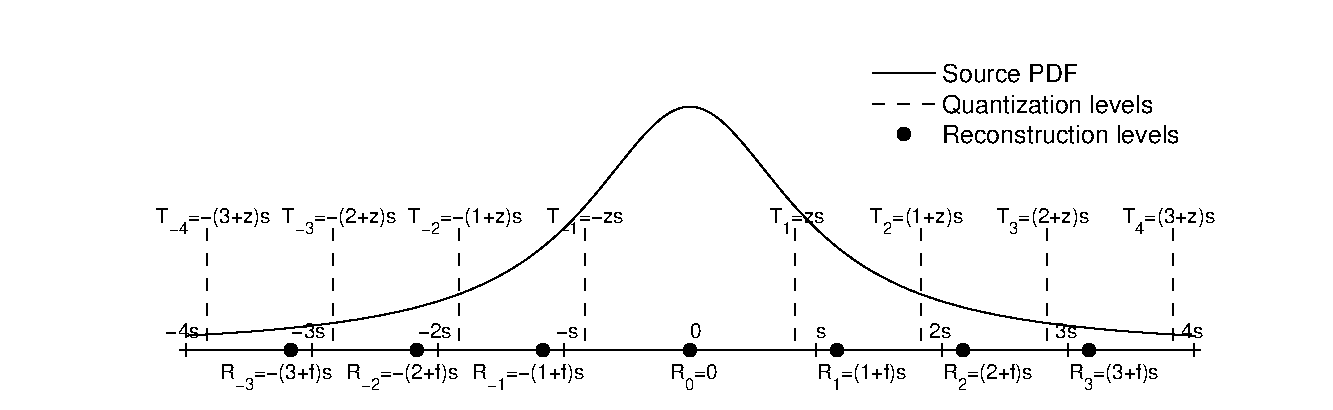
\includegraphics[width = 1.0\linewidth]{Figures/section2/DZ+UTSQ_NURQ}\\
\caption{\label{fig:DZ+UTSQ_NURQ}%
Illustration of DZ+UTSQ/NURQ Scheme.}
\vspace{5pt}
\end{figure}

\subsection{Problem Formulation of R-D Analysis}
For random variable $X$ conforming to source distribution $p(x)$, when applying high-resolution DZ+UTSQ/NURQ scheme, after DZ+UTSQ classification process, the entropy can be denoted by the \emph{R-Q function} (RQF):
\begin{equation}\label{equ:formula-rq}
	H(z, s) = \sum_{i=-\infty}^{+\infty} H_i
	= -\sum_{i=-\infty}^{+\infty} P_i \log_2 P_i ,
\end{equation}
where $H_k = - P_k \log_2 P_k$ is the entropy of quantization interval $I_k$, whereas $P_k$ is the possibility of $X$ belongs to quantization interval $I_{k}$:
\begin{equation}\label{equ:formula-pk}
	P_k = P\{X \in I_k\} =
	\begin{cases}
		\int_{-z s}^{z s} p(x) dx
		= 2 \int_{0}^{z s} p(x) dx,
		& k=0 \\
		\int_{(k-1+z) s}^{(k+z) s} p(x) dx,
		& k \ge 1 \\
		P_{-k},
		& k \le -1 .
	\end{cases}
\end{equation}  

Likewise, after NURQ reconstruction process, the reconstruction error under MSE criterion can be denoted by the \emph{D-Q function} (DQF):
\begin{equation}\label{equ:formula-dq}
	E(z, s, p) =\sum_{i=-\infty}^{+\infty} E_i
	=E_0 + 2 \sum_{i=1}^{+\infty} E_i ,
\end{equation}
where $E_k$ is the reconstruction error generated in quantization interval $I_k$:
\begin{equation}\label{equ:formula-dk}
	E_k=
	\begin{cases}
		\int_{-z s}^{z s} |x|^2 p(x) dx,
		& k=0 \\
		\int_{(k-1+z) s}^{(k+z) s} |x - (k+f) s|^2 p(x) dx,
		& k \ge 1 \\
		E_{-k},
		& k \le -1 .
	\end{cases}
\end{equation}

Although the RQF and DQF provide a way to calculate rate and distortion, however, for most source distributions, when the sophisticated PDFs (e.g. the exponential form for GGD and power form for Cauchy) are combined with DZ+UTSQ/NURQ, it is incapable to directly obtain the closed-form RQF and DQF from (\ref{equ:formula-rq}) - (\ref{equ:formula-dk}), not to mention deriving the accurate R-D relationship from RQF and DQF. In the following sections, we turn to decouple the R-D analysis problem by investigating the respective influence of source distribution and quantizer design on R-D performance, which can bring new insight and inspiration towards R-D research of image/video applications. 

\section{A Universal R-D Property of General Source Distributions}
%In this section, we provide theoretical analysis and rigorous validations to reveal a universal R-D property of general sources: for any source distribution that can be expressed as the product of a SF and its RP, the SF does not affect its derivative R-D function. Without loss of generality, in this paper, we mainly use PSNR as the criterion of objective distortion, and for other distortion measure like MSE, the results can be easily derived via simple calculation.
%\SubSection{Theoretical Analysis}
In this section, we provide theoretical analysis to reveal a universal R-D property of general sources: for any source distribution that can be expressed as the product of a SF and its RP, the SF does not affect its derivative R-D function.

For any given general source distribution satisfying (\ref{equ:SF}), the original PDF $p(x)$ can be expressed as the product of a SF $c$ and RP $q(x)$. Accordingly, for quantization step $s$, a new variable $\delta$ can be found satisfying $\delta = s/c$. By using $1/c \cdot q(x/c)$ to replace $p(x)$ and $c \cdot \delta$ to replace $s$, the RQF and DQF can be expressed in a new form. First, for RQF, (\ref{equ:formula-pk}) can be rewritten as:
\begin{equation}\label{equ:formula-pknew}
	P_k =
	\begin{cases}
		\int_{-z c\delta}^{z c\delta} q\left(\frac{x}{c}\right) d\left(\frac{x}{c}\right)
		= 2 \int_{0}^{z \delta} q(x) dx,
		& k=0 \\
		\int_{(k-1+z) c\delta}^{(k+z) c\delta} q\left(\frac{x}{c}\right) d\left(\frac{x}{c}\right)
		=\int_{(k-1+z) \delta}^{(k+z) \delta} q(x) dx,
		& k \ge 1 \\
		P_{-k},
		& k \le -1 ,
	\end{cases}
\end{equation} 
where $\delta$ and $z$ are function variables and $q(x)$ is integrand. According to (\ref{equ:formula-rq}), the overall entropy and the entropy for each quantization interval $I_k$ are only determined by $\delta$ and $z$, being irrelevant to $c$. Specifically, given the constant dead-zone ratio $z$, the RQF is just a function of $\delta$: 
\begin{equation}\label{equ:formula-rqnew}
	H = R_z(\delta).
\end{equation}

\begin{figure}[tp]
\begin{center}
\begin{tabular}{cc}
%\multicolumn{2}{c}{\includegraphics[width = 0.6\linewidth]{Figures/image1}} \\
%\multicolumn{2}{c}{\small{(a)}} \\[1em]
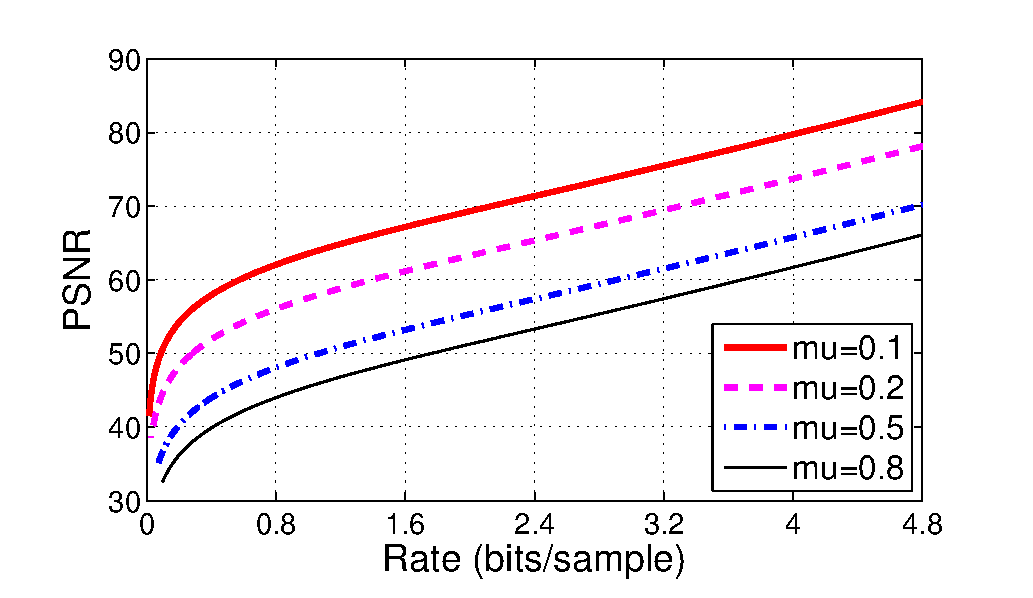
\includegraphics[width = 0.5\linewidth]{Figures/section3/RD_Cauchy_z=0_75_p=0} &
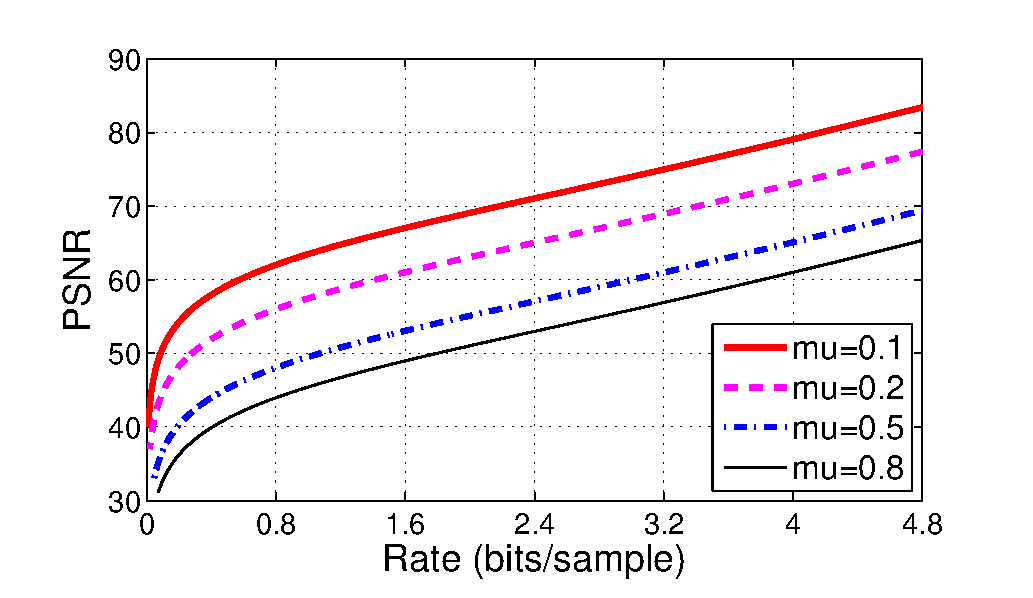
\includegraphics[width = 0.5\linewidth]{Figures/section3/RD_Cauchy_z=0_89_p=0_33} \\
{\small (a) $z=3/4,\;f=0$} & {\small (b) $z=8/9,\;f=1/3$} \\
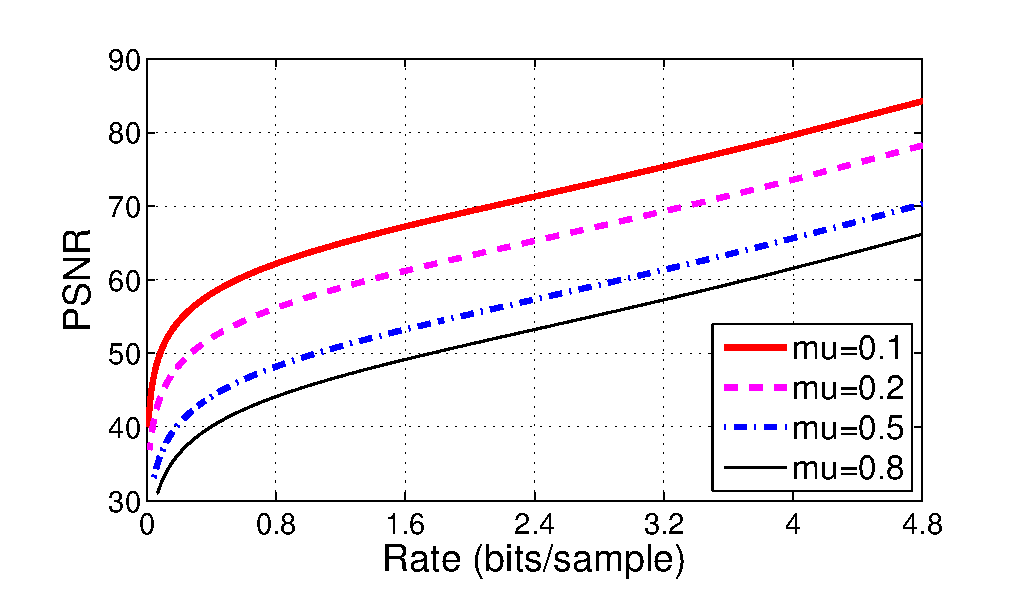
\includegraphics[width = 0.5\linewidth]{Figures/section3/RD_Cauchy_z=1_2_p=0_57} &
\includegraphics[width = 0.5\linewidth]{Figures/section3/RD_Cauchy_z=1_p=0_5} \\
{\small (c) $z=5/6,\;f=4/7$} & {\small (d) $z=1,\;f=1/2$} 
\end{tabular}
\end{center}
\vspace{-20pt}
\caption{\label{fig:RD_mu}
Cauchy PSNR-R curves for different $\mu$ under DZ+UTSQ/NURQ.}
\end{figure} 

Similarly, for DQF, (\ref{equ:formula-dk}) can be rewritten as:  
\begin{equation}\label{equ:formula-dknew}
	E_k =
	\begin{cases}
		\int_{-z c\delta}^{z c\delta} |x|^2 q\left(\frac{x}{c}\right) d\left(\frac{x}{c}\right)
		= c^2\int_{-z \delta}^{z \delta} |x|^2 q(x) d(x),
		& k=0 \\
		\int_{(k-1+z) c\delta}^{(k+z) c\delta} |x - (k+f) c\delta|^2 q\left(\frac{x}{c}\right) d\left(\frac{x}{c}\right)\\
		=c^2\int_{(k-1+z) \delta}^{(k+z) \delta} |x - (k+f) \delta|^2 q(x) dx,
		& k \ge 1 \\
		E_{-k},
		& k \le -1 .
	\end{cases}
\end{equation} 
For convenience, we define $F_k$ as:
\begin{equation}\label{equ:formula-fk}
	F_k =
	\begin{cases}
		= \int_{-z \delta}^{z \delta} |x|^2 q(x) d(x),
		& k=0 \\
		=\int_{(k-1+z) \delta}^{(k+z) \delta} |x - (k+f) \delta|^2 q(x) dx,
		& k \ge 1 \\
		F_{-k},
		& k \le -1 .
	\end{cases}
\end{equation} 
Thus, we have $E_k = c^2 F_k$, where $F_k$ is only determined by $\delta, z$ and $f$, being irrelevant to $c$. According to (\ref{equ:formula-dq}), given the constant $z$ and $f$, the DQF can be regarded as a function of $\delta$ with the coefficient of $c^2$:
\begin{equation}\label{equ:formula-dqnew}
	E = c^2 \sum_{i=-\infty}^{+\infty} F_i = c^2 D_{z,f}(\delta).
\end{equation}
Moreover, using PSNR criterion, the DQF is expressed as:
\begin{equation}\label{equ:formula-dqpsnr}
	\textrm{PSNR} =\frac{-10}{\ln{10}}\frac{1}{D_{z,f}(\delta)}\frac{\partial D_{z,f}(\delta)}{\partial\delta}.
\end{equation}

With (\ref{equ:formula-rqnew}) and (\ref{equ:formula-dqpsnr}), it is easy to see that the derivative of RQF and DQF with respect to $\delta$, i.e. $\partial H / \partial \delta$ and $\partial PSNR / \partial \delta$, are irrelevant to $c$. Based on the derivative method for compound functions, we have: 
\begin{equation}\label{equ:formula-derivativedr}
	\frac{\partial\textrm{PSNR}}{\partial H} = \frac{\frac{\partial\textrm{PSNR}}{\partial\delta}}{\frac{\partial H}{\partial\delta}} 
	= \frac{-10}{\ln{10}}\frac{1}{D_{z,f}(\delta)}\frac{\partial D_{z,f}(\delta)}{\partial R_{z}(\delta)} ,
\end{equation} 
which indicates the derivative PSNR-R function of the source distribution is not affected by its SF.

\begin{figure}[tp]
\begin{center}
\begin{tabular}{cc}
\includegraphics[width = 0.5\linewidth]{Figures/section3/RDDerivative_Cauchy_z=0_75_p=0} &
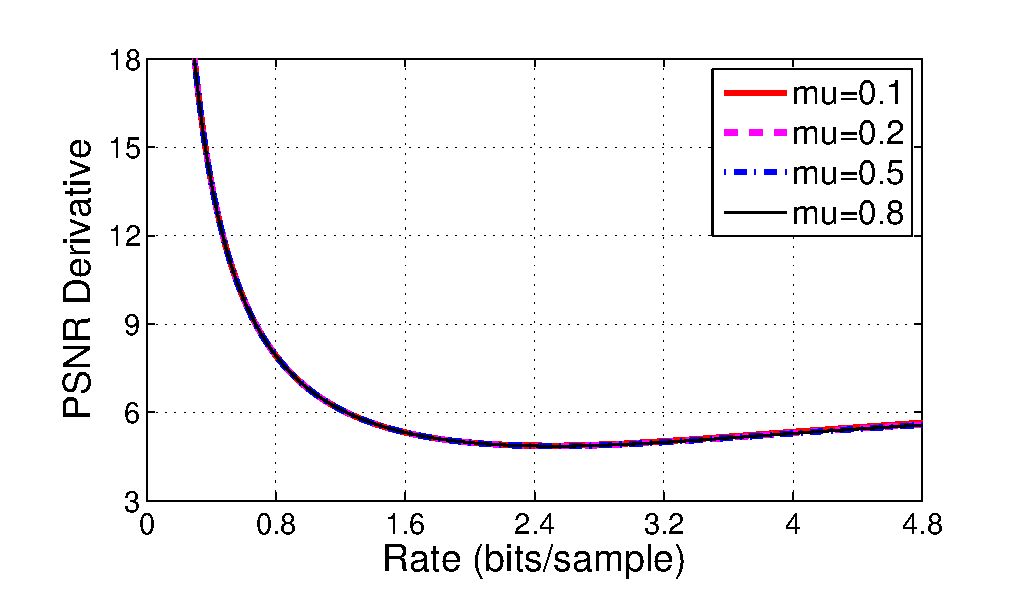
\includegraphics[width = 0.5\linewidth]{Figures/section3/RDDerivative_Cauchy_z=0_89_p=0_33} \\
{\small (a) $z=3/4,\;f=0$} & {\small (b) $z=8/9,\;f=1/3$} \\
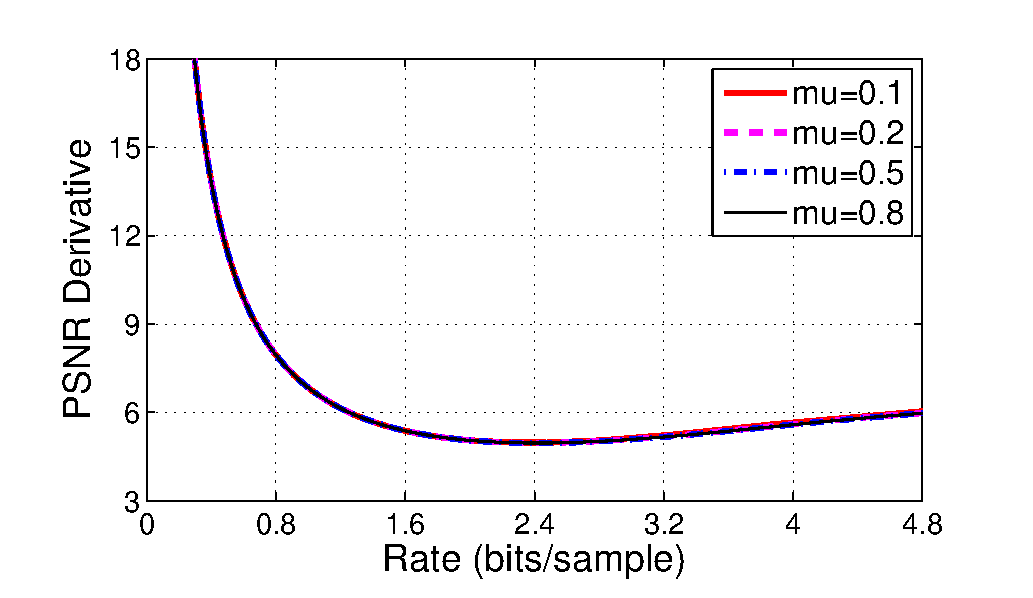
\includegraphics[width = 0.5\linewidth]{Figures/section3/RDDerivative_Cauchy_z=1_2_p=0_57} &
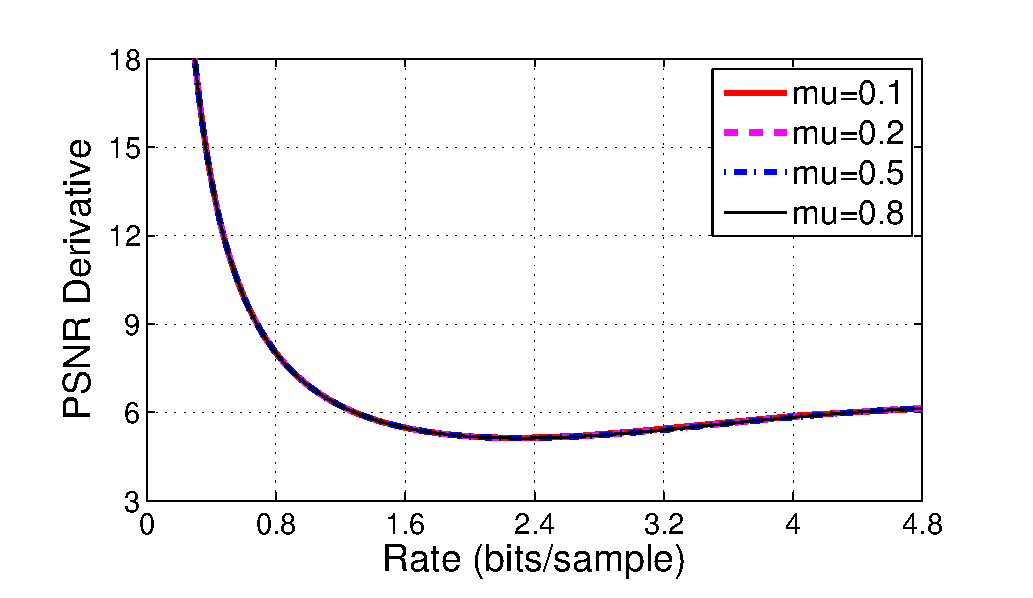
\includegraphics[width = 0.5\linewidth]{Figures/section3/RDDerivative_Cauchy_z=1_p=0_5} \\
{\small (c) $z=5/6,\;f=4/7$} & {\small (d) $z=1,\;f=1/2$} 
\end{tabular}
\end{center}
\vspace{-20pt}
\caption{\label{fig:RDDerivative_mu}
Cauchy derivative PSNR-R curves for different $\mu$ under DZ+UTSQ/NURQ.}
\end{figure} 

The irrelevance of SF to derivative R-D function is a universal property applicable to any source distribution satisfying (\ref{equ:SF}), and we can easily verify this property on GGD and Cauchy distributions which are commonly-used in modeling real video and image source signals. For GGD, in our previous work \cite{Sun_TIP2013}, the SF $\beta$ is theoretically proved not relative to the derivative PSNR-R function, which is also confirmed via extensive simulation results. For Cauchy distribution, under DZ+UTSQ/NURQ scheme, the curves of PSNR-R function and its derivative are illustrated in Fig. \ref{fig:RD_mu} and Fig. \ref{fig:RDDerivative_mu}, respectively. From Fig. \ref{fig:RD_mu}, the curves corresponding to four SF values $\mu = 0.2, 0.5, 0.8 \; \textrm{and} \; 1.0$ are observed perfectly overlapped in all bitrate range. Therefore, different $\mu$ do not change the shape of PSNR-R function of Cauchy distribution, but only lead to the parallel displacement of the PSNR-R curve, as is shown in Fig. \ref{fig:RDDerivative_mu}. With the influence of SF on R-D performance clearly identified, the complexity of R-D analysis problem for further research and application can be properly reduced. 

%\SubSection{Validation of R-D Property in GGD and Cauchy Distribution}
%For GGD, the SF is $\beta$ which is also regarded as the GGD standard deviation. In our previous work [??], we theoretically proved the existence of the derivative RQF and DQF with respect to $\delta$, and then deduced that $\beta$ is not relative to the derivative D-R function of GGD, which is also confirmed via the illustrations of extensive simulation results. Here, we mainly focus on Cauchy distribution where the SF is $\mu$ and RP is $1 / \pi (1+x^2)$. For Cauchy distribution, the existence of its derivative RQF can be theoretically proved using similar approaches in [??], where as for DQF, since Cauchy distribution does not have variance and expectation, the overall reconstruction error under high-resolution DZ+UTSQ/NURQ scheme cannot be calculated. However, in practice, the number of quantization interval is limited, thus the DQF and its derivative can be approximated using numerical simulation. In Figure. ?? the D-R derivative curves of Cauchy distribution with $\mu = 0.2, 0.5, 0.8 and 1.0$ under four different DZ+UTSQ quantizers are illustrated, from which the D-R derivative curves with different $\mu$ are observed perfectly overlapped, indicating that the SF of Cauchy distribution does not affect its derivative R-D function. As is illustrated in Figure ??, different $\mu$ only lead to the parallel displacement of the entire curve of D-R function for Cauchy distribution. 

%Therefore, for each integer $k$, both $P_k$ and its derivative with respect to $\delta$, i.e. $\partial P_k / \partial \delta$, are irrelevant to $c$. Since the entropy $H_k$ of quantization interval $I_k$ equals to $- P_k \log_2 P_k$ which is convergent when $\delta > 0$, it is clear that both $H_k$ and $\partial H_k / \partial \delta$ are irrelevant to $c$, indicating that $ \sum_{k=-\infty}^{+\infty} H_k$ and $\sum_{k=-\infty}^{+\infty} \frac{\partial H_k}{\partial \delta}$ are both irrelevent to $c$. If the infinite series $\sum_{k=-\infty}^{+\infty} \frac{\partial H_k}{\partial \delta}$ is continuous and uniform convergent, according to (\ref{equ:formula-rq}), the derivative of overall entropy $H$ on $\delta$, i.e. $\partial H / \partial \delta$ exists, which is irrelevant to $c$.


\section{Efficient DZ+UTSQ/NURQ Design Principles for Various Sources}

For general sources, the necessary conditions for quantizer design to achieve optimum R-D performance were formulated in \cite{Farvardin_TIT1984}. Specifically, under MSE criterion, Max \cite{Max_TIT1960} obtained the famous conclusion that, for each quantization index $k$, the reconstruction level $R_k$ should locate at the \emph{centroid} of the PDF $p(x)$ within quantization interval $I_k$. Thus, for symmetric DZ+UTSQ/NURQ scheme, the optimum design requires:
\begin{equation}\label{equ:formula-OptQuant}
	{R_k}^* = \int_{(k-1+z)s}^{(k+z)s} xp(x)dx / \int_{(k-1+z)s}^{(k+z)s} p(x)dx, \quad k \ge 1,
\end{equation}
whereas for $k \le 0$ the results can be similarly deduced without loss of generality. Based on (\ref{equ:DZ+UTSQ/NURQ}) and (\ref{equ:formula-OptQuant}), for all types of distributions, the preliminary constraint on $z$ and $f$ of efficient DZ+UTSQ/NURQ design is deduced: 
\begin{equation}\label{equ:formula-PreConstraint}
	 0 < z - f \le 1. 
\end{equation}

\begin{figure}[tp]
\centering
\includegraphics[width = 0.95\linewidth]{Figures/section4/DZ+UTSQ_NURQ_linear_constraint}\\
\caption{\label{fig:linear_constraint}
Two DZ+UTSQ/NURQ designs that satisfy the necessary condition of optimal R-D performance for heavy-tailed distribution.}
% \vspace{5pt}
\end{figure}

Then we narrow the source distribution types to the widely-used source models of the real video/image signals. For these sources, the PDF is always zero-mean and monotonically decreasing in positive axis. With this feature, it is easy to prove:
\begin{equation}\label{equ:formula-Inequity1}
	\int_{(k-1+z)s}^{(k+z)s} xp(x)dx \le (k+z-\frac{1}{2}) s \int_{(k-1+z)s}^{(k+z)s} p(x)dx, \quad k \ge 1.
\end{equation}
By integrating (\ref{equ:formula-OptQuant}) and (\ref{equ:formula-Inequity1}), it is clear that:
\begin{equation}\label{equ:formula-Inequity2}
	{R_k}^* \le (k+z-\frac{1}{2}), \quad k \ge 1.
\end{equation}
From (\ref{equ:DZ+UTSQ/NURQ}) and (\ref{equ:formula-Inequity2}), the preliminary constraint (\ref{equ:formula-PreConstraint}) can be refined as:
\begin{equation}\label{equ:formula-RefConstraint}
	\frac{1}{2} \le z - f \le 1. 
\end{equation}

\begin{figure}[tp]
\begin{center}
\begin{tabular}{cc}
\includegraphics[width = 0.5\linewidth]{Figures/section4/RD_Cauchy_mu=0_5_z=p+0_5} &
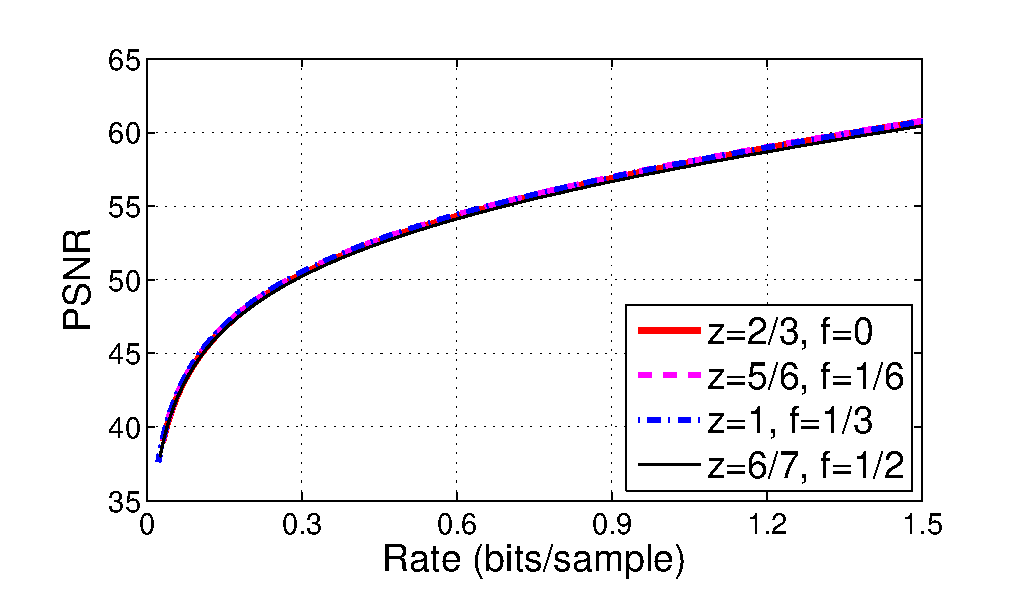
\includegraphics[width = 0.5\linewidth]{Figures/section4/RD_Cauchy_mu=0_5_z=p+0_67} \\
{\small (a) $z=p+1/2$} & {\small (b) $z=p+2/3$} \\
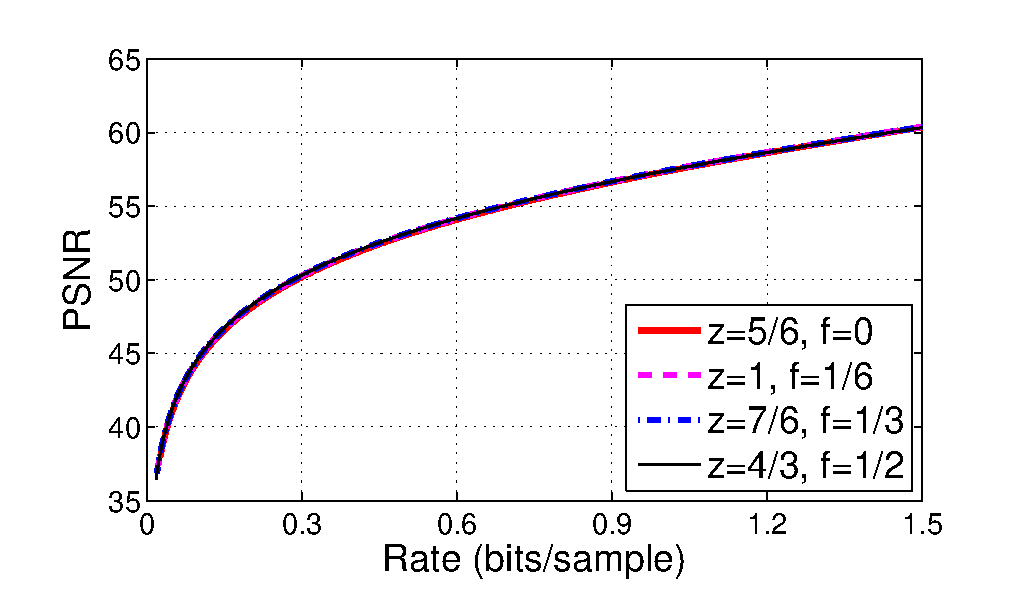
\includegraphics[width = 0.5\linewidth]{Figures/section4/RD_Cauchy_mu=0_5_z=p+0_83} &
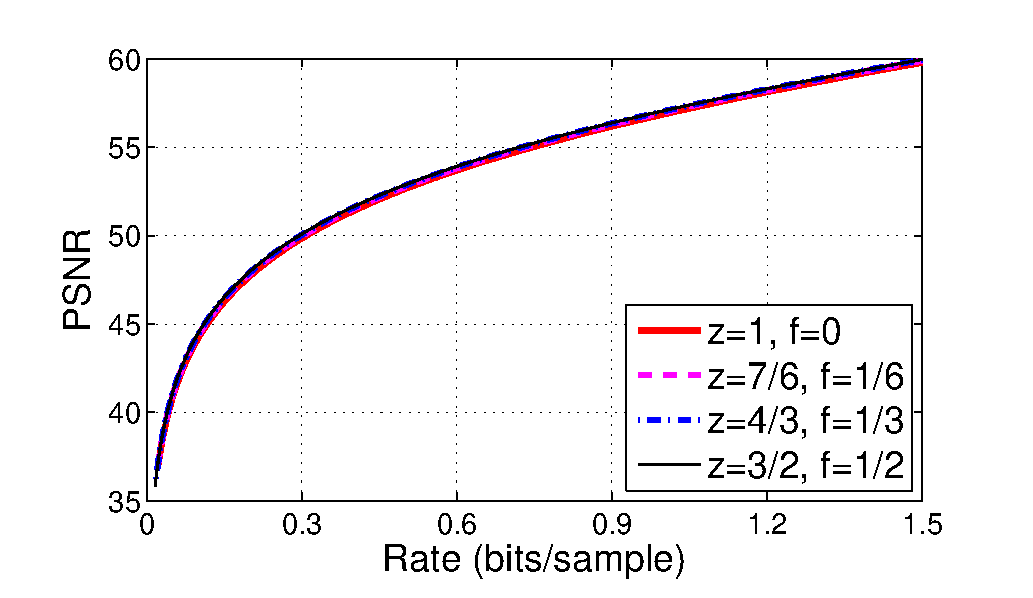
\includegraphics[width = 0.5\linewidth]{Figures/section4/RD_Cauchy_mu=0_5_z=p+1} \\
{\small (c) $z=p+5/6$} & {\small (d) $z=p+1$} 
\end{tabular}
\end{center}
\vspace{-20pt}
\caption{\label{fig:RD_same_pattern}
R-D performance comparison of different quantizer designs conforming to the same DZ+UTSQ/NURQ linear pattern satisfying (\ref{equ:formula-LinearConstraint}) for Cauchy $\mu=0.5$.}
\end{figure} 

Particularly, when the source distribution types are further specified as some zero-mean heavy-tailed distribution \footnote{http://en.wikipedia.org/wiki/Heavy-tailed\_distribution}, e.g. Cauchy distribution, the refined constraint (\ref{equ:formula-RefConstraint}) can be more accurately described. Consider the quantization interval $I_k$ ($k > 0$), where the reconstruction level $R_k$ divides $I_k$ into two parts: $\overline{T_k R_k}$ and $\overline{R_k T_{k+1}}$. Since Cauchy distribution provides a useful model of broad-tailed stochastic phenomena \cite{Farvardin_TIT1984}, in quantization intervals other than dead-zone ($\forall I_k, \; k \ne 0$), the PDF of Cauchy distribution can be precisely approximated as a straight line, as is shown in Fig. \ref{fig:linear_constraint}. Thus, when the slope of PDF in $I_k$ is fixed, according to the necessary condition (\ref{equ:formula-OptQuant}), to keep $R_k$ the centroid of PDF in $I_k$, the distance ratio of $\overline{T_k R_k} / \overline{R_k T_{k+1}}$ should remain constant. To make it clear, efficient DZ+UTSQ/NURQ design requires two different patterns $z_1, f_1$ and $z_2, f_2$ to satisfy:
\begin{equation}\label{equ:formula-ratio}
\frac{(k+f_1)-(k-1+z_1)}{(k+z_1)-(k+f_1)} = \frac{(k+f_2)-(k-1+z_2)}{(k+z_2)-(k+f_2)},
\end{equation}
which means $z_1 - z_2 = f_1 - f_2$, indicating $z$ and $f$ should be linear correlate. Therefore, based on the refined constraint (\ref{equ:formula-RefConstraint}), a linear constraint on $z$ and $f$ is derived:
\begin{equation}\label{equ:formula-LinearConstraint}
	z = f+c, \quad \frac{1}{2} \le c \le 1, 
\end{equation}
where $c$ is constant real number.

\begin{figure}[tp]
\begin{center}
\begin{tabular}{cc}
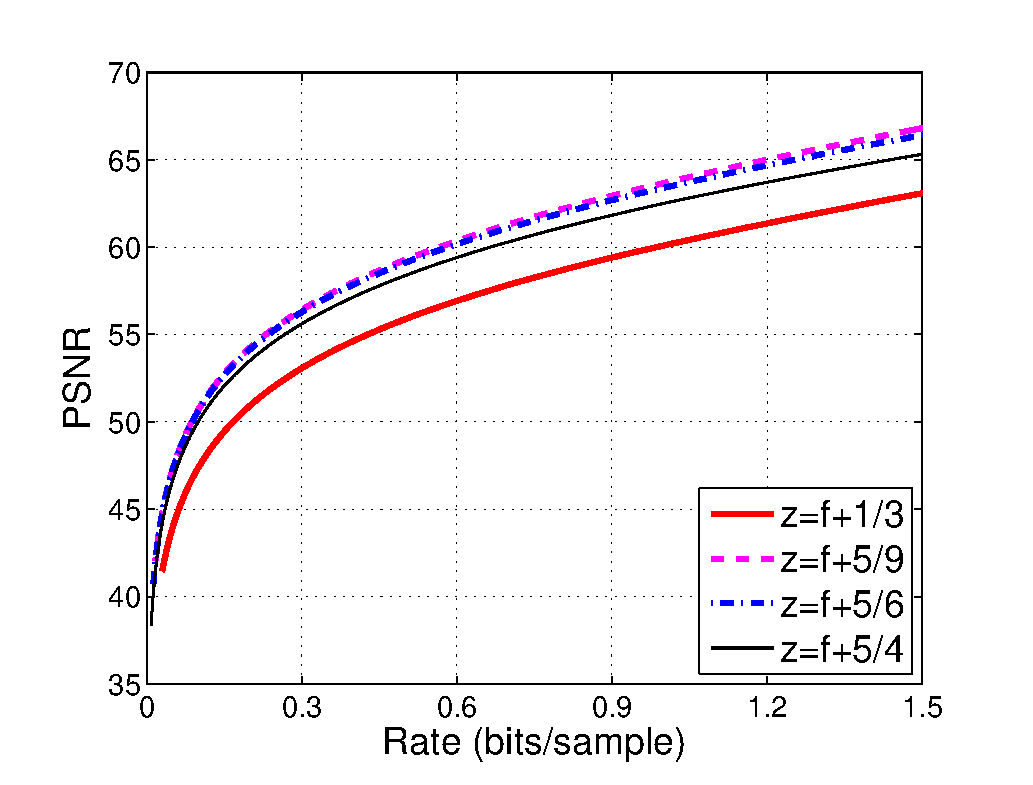
\includegraphics[width = 0.5\linewidth]{Figures/section4/RD_Cauchy_mu=0_2_linear_patterns} &
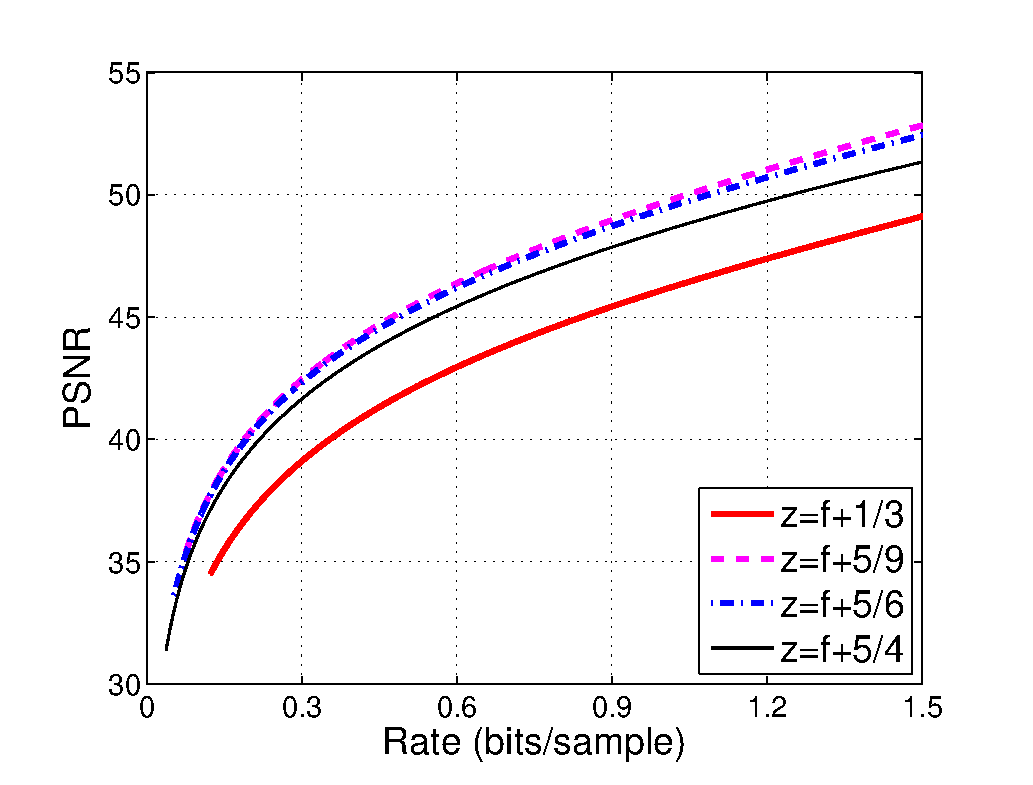
\includegraphics[width = 0.5\linewidth]{Figures/section4/RD_Cauchy_mu=0_8_linear_patterns} \\
{\small (a) Cauchy $\mu=0.2$} & {\small (b) Cauchy $\mu=0.8$}
\end{tabular}
\end{center}
\vspace{-20pt}
\caption{\label{fig:RD_different_patterns}
R-D performance comparison of different DZ+UTSQ/NURQ linear patterns, which reflects the superiority of the patterns satisfying (\ref{equ:formula-LinearConstraint}).}
\end{figure} 

Deduced from the necessary condition (\ref{equ:formula-OptQuant}), in actual bitrate ($0-1.5$ bits/sample), the linear constraint (\ref{equ:formula-LinearConstraint}) is an efficient principle to evaluate the R-D performance of different DZ+UTSQ/NURQ designs, which can be reflected via two groups of simulation experiments on Cauchy distribution. The first group of experiments are designed to show that the linear constraint is a precise performance classifier of DZ+UTSQ/NURQ. Related results for $\mu = 0.5$ are exhibited in Fig. \ref{fig:RD_same_pattern}. From the R-D performance comparison of different DZ+UTSQ/NURQ designs, it is observed that, under each linear pattern, all the PSNR-R curves are exactly overlapped with each other, indicating the identical R-D performance of different DZ+UTSQ/NURQ designs conforming to the same linear pattern satisfying (\ref{equ:formula-LinearConstraint}). The second group of experiments are designed to show that the linear constraint is also an accurate indicator of superior R-D performance. Related results for $\mu = 0.2$ and $0.8$ are exhibited in Fig. \ref{fig:RD_different_patterns}. From the R-D performance comparison of different linear patterns, it is obvious that only the linear patterns satisfying (\ref{equ:formula-LinearConstraint}) can achieve desirable R-D performance.

It should be noted that, as an efficient DZ+UTSQ/NURQ design principle, the linear constraint (\ref{equ:formula-LinearConstraint}) is not only applicable for Cauchy distribution but also for a big class of zero-mean heavy-tailed distributions (requiring monotonic PDF in positive axis). Actually, even for GGD, this constraint is a good R-D performance evaluator, as is shown in our previous work \cite{Sun_TIP2013}. However, since GGD has faster, exponential rate of decay, for GGD, different DZ+UTSQ/NURQ designs conforming to the same linear pattern of $z$ and $f$ may have slight deviation in R-D performance. 

In sum, the constraints (\ref{equ:formula-PreConstraint}), (\ref{equ:formula-RefConstraint}) and (\ref{equ:formula-LinearConstraint}) provide a convenient way to simplify the R-D performance analysis of various different source distributions. Benefiting from these principles, the reason why the DZ+UTSQ/NURQ designs applied in video/image coding standards (e.g. in H.264/AVC, $z$ is set to $2/3$ in intra coding and $5/6$ in inter coding, $f$ is set to $0$ \cite{Sullivan_VCIP2005}) are effective can now be theoretically explained.

\section{Conclusion}

In this paper, a novel study is performed to reveal the respective influence of source distributions and quantizer design on R-D performance. First, the property of general sources under DZ+UTSQ/NURQ is discovered to identify the irrelevance of SF to the derivative R-D function, which properly reduces the complexity of the R-D analysis problem. Second, by taking the features of source distributions into account, efficient DZ+UTSQ/NURQ design principles are deduced for different types of sources, which can be used to conveniently evaluate the R-D performance of various different quantizer patterns. These contributions can bring new insight and inspiration towards the R-D research for video/image applications.

% \begin{figure}[h]
% \begin{center}
% \begin{tabular}{cc}
% \multicolumn{2}{c}{\includegraphics[width = 0.6\linewidth]{Figures/image1}} \\
% \multicolumn{2}{c}{\small{(a)}} \\[1em]
% \includegraphics[width = 0.3\linewidth]{Figures/image3} &
% \includegraphics[width = 0.3\linewidth]{Figures/image4} \\
% {\small (b)} & {\small (c)}
% \end{tabular}
% \end{center}
% \caption{\label{fig:example}%
% An example figure.}
% \end{figure}

% \begin{table}[htp]
% \begin{center}
% \caption{\label{tab:example}%
% Average PSNR in dB for the ``Coastguard'' video sequence}
% {
% \renewcommand{\baselinestretch}{1}\footnotesize
% \begin{tabular}{|c|c|c|c|c|}
% \cline{2-5}
% \multicolumn{1}{c|}{~}&
% \multicolumn{1}{c|}{2D} &
% \multicolumn{1}{c|}{3D} &
% \multicolumn{2}{c|}{MC-BCS-SPL}\\
% \cline{4-5}
% \multicolumn{1}{c|}{$S_{\text{NK}}$} &
% BCS-SPL & BCS-SPL & $S_{\text{K}}=S_{\text{NK}}$ & $S_{\text{K}}=0.7$\\
% \hline
% 0.1 &22.69 &22.76 &23.06 &25.29 \\
% 0.2 &24.70 &24.76 &25.78 &27.94 \\
% 0.3 &26.37 &26.45 &28.29 &30.15 \\
% 0.4 &27.99 &27.95 &30.88 &32.30 \\
% 0.5 &29.60 &29.57 &33.58 &34.42 \\
% \hline
% \end{tabular}}
% \end{center}
% \end{table}

\section*{References}
\bibliographystyle{IEEEtran}
\bibliography{refs}

[Sullivan\_IEEE2005]Sullivan, Gary J., and Thomas Wiegand. "Video compression-from concepts to the H. 264/AVC standard." Proceedings of the IEEE 93.1 (2005): 18-31.

[Hang\_TCSVT1997]H.-M. Hang and J.-J. Chen, “Source model for transform video coder
and its application. I. Fundamental theory,” IEEE Trans. Circuits Syst.
Video Technol., vol. 7, no. 2, pp. 287–298, Apr. 1997.

[Kamaci\_TCSVT2005]N. Kamaci, Y. Altunbasak, and R. M. Mersereau, “Frame bit allocation for the H.264/AVC video coder via Cauchy-density-based rate and distortion models,” IEEE Trans. Circuits Syst. Video Technol., vol. 15, no. 8, pp. 994–1006, Aug. 2005.

[Rodríguez\_TCSVT2010]Sanz-Rodríguez, S., del-Ama-Esteban, Ó., de-Frutos-López, M., Díaz-de-María, F. (2010). Cauchy-density-based basic unit layer rate controller for H. 264/AVC. Circuits and Systems for Video Technology, IEEE Transactions on, 20(8), 1139-1143.

[Sun\_TIP2013]Sun, Jun, Yizhou Duan, Jiangtao Li, Jiaying Liu, and Zongming Guo. "Rate-Distortion Analysis of Dead-Zone Plus Uniform Threshold Scalar Quantization and Its Application—Part I: Fundamental Theory." Image Processing, IEEE Transactions on 22, no. 1 (2013): 202-214.

[Smooth\_SPIE1996]S. R. Smooth and R. A. Lowe, “Study of DCT coefficients distributions,” Proc. SPIE , pp. 403-311, Jan. 1996.
[Pratt\_Wiley1978]W. K. Pratt, “Digital Image Processing,” New York: Wiley-Interscience, 1978, ch. 10.

\end{document}
